\documentclass[tikz]{standalone}

\usepackage{tikz}
\usetikzlibrary{arrows.meta}
\usetikzlibrary{decorations.pathreplacing}

% For tables
\usepackage{booktabs}

% For dashed lines
\usepackage{arydshln}

\begin{document}

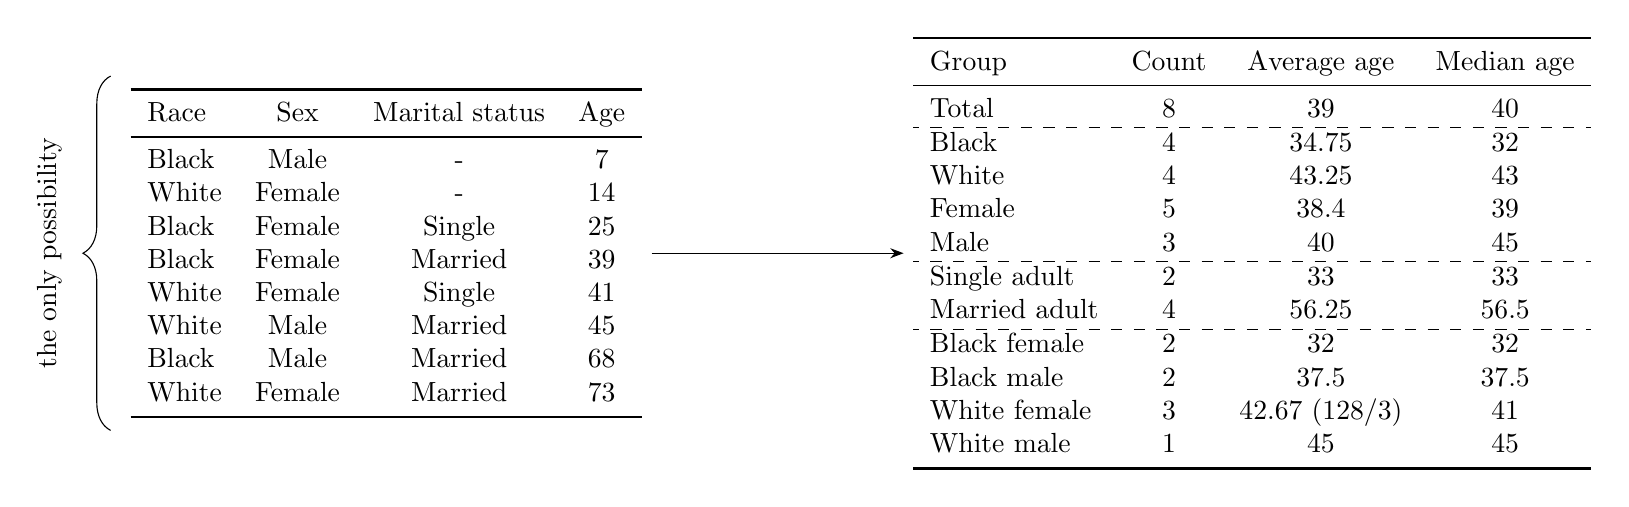
\begin{tikzpicture}[>=Stealth]
  \node (individuals-table) at (0, 0) {%
      \begin{tabular}{lccc}
	\toprule
	Race & Sex & Marital status & Age \\
	\midrule
	Black & Male   & -       & 7  \\
	White & Female & -       & 14 \\
	Black & Female & Single  & 25 \\
	Black & Female & Married & 39 \\
	White & Female & Single  & 41 \\
	White & Male   & Married & 45 \\
	Black & Male   & Married & 68 \\
	White & Female & Married & 73 \\
	\bottomrule
      \end{tabular}
    };

  \node (summary-table) at (11, 0) {%
      \begin{tabular}{lccc}
	\toprule
	Group & Count & Average age & Median age \\
	\midrule
	Total         & 8 & 39              & 40   \\
	\hdashline
	Black         & 4 & 34.75           & 32   \\
	White         & 4 & 43.25           & 43   \\
	Female        & 5 & 38.4            & 39   \\
	Male          & 3 & 40              & 45   \\
	\hdashline
	Single adult  & 2 & 33              & 33   \\
	Married adult & 4 & 56.25           & 56.5 \\
	\hdashline
	Black female  & 2 & 32              & 32   \\
	Black male    & 2 & 37.5            & 37.5 \\
	White female  & 3 & 42.67 ($128/3$) & 41   \\
	White male    & 1 & 45              & 45 \\
	\bottomrule
      \end{tabular}
    };

  \draw[->] (individuals-table) -- (summary-table);

  \draw [decorate,decoration={brace, amplitude=10pt, mirror}, yshift=0pt] (-3.5, 2.25) -- node[rotate=90, above, yshift=0.5cm] {the only possibility} (-3.5, -2.25);

\end{tikzpicture}

\end{document}
